\section{Proposition de l'article}

Le modèle de segmentation par contour actif utilisant le champ GVF pour définir son énergie externe présente cependant des limitations dont Bing Li \& al font mention dans leur article : un temps de calcul important, une forte sensibilité au bruit et aux paramètres. D'autre part, la relation entre les paramètres de GVF et la portée à laquelle le contour actif est attirée par le bord n'est pas claire.\\

Afin de corriger ces différents problèmes, Bing Li \& al présentent dans cet article une nouvelle définition de la force externe régissant l'évolution du contour actif vers les bords  de l'objet à segmenter. Cette nouvelle force externe, nommé Vector Field Convolution (VFC), est calculée en convoluant un noyau de champ de vecteur à une carte des contours extraite de l'image d'origine.   

\subsection{Minimisation de l'énergie $E_{ac}$}

Lorsque le minimum de $E_{ac}$ est atteint, le contour actif $\mathbf{v}(s)$ doit satisfaire l'équation d'Euler-Lagrange :
\begin{equation}
	\alpha \mathbf{v}'' - \beta \mathbf{v}'''' + f_{ext}(\mathbf{v}) = 0
	\label{eq:bilan}
\end{equation}

où $f_{ext}= - \nabla E_{ext}(\mathbf{v})$

Cette équation, qui peut être vue comme une équation bilan des forces internes ($\alpha \mathbf{v}'' - \beta \mathbf{v}''''$) et externes $f_{ext}$, permet de calculer $\mathbf{v}(s)$. Afin de résoudre \ref{eq:bilan}, le contour $\mathbf{v}(s)$ est considéré comme une fonction du temps $t$. La solution est obtenue en appliquant une descente de gradient sur l'équation en partant d'un contour initial $\mathbf{v}(s,0)$:

\begin{equation}
	\frac{\partial \mathbf{v}(s,t)}{\partial t} = \alpha \mathbf{v}''(s,t) - \beta \mathbf{v}''''(s,t)+f_{ext}(\mathbf{v}(s,t))
	\label{eq:graddesc}
\end{equation}

Cette équation est ensuite résolue numériquement en utilisant une approche par différence finie (besoin d'en parler ??).

Bing Lie \& al remplace dans leur article la force externe $f_{ext}(\mathbf{v})$ par le champ VFC $f_{vfc}(\mathbf{v})$ dans l'équation \ref{eq:graddesc}.

\subsection{Vector Field Convolution}

Afin de calculer cette nouvelle force externe statique, les auteurs définissent d'abord un \textit{vector field kernel} $\mathbf{k}(x,y)=[u_k(x,y),v_k(x,y)]$ tel que chaque vecteur pointe vers l'origine du noyau 
\begin{equation}
	\mathbf{k}(x,y)=m(x,y)\mathbf{n}(x,y)
\end{equation}
où $m(x,y)$ est le poids affecté au vecteur en $(x,y)$ et $\mathbf{n}(x,y)$ est le vecteur unitaire pointant vers l'origine du noyau $(0,0)$.

A partir du noyau $\mathbf{k}(x,y)$ et de la carte des contours $F(x,y)$ obtenue à partir de l'image d'origine $I(x,y)$, le champ VFC est définie par :

\begin{align*}
	f_{vfc}(x,y) & = F(x,y)*\mathbf{k}(x,y) \\
				 & = [F(x,y)*u_k(x,y),F(x,y)*v_k(x,y)]
\end{align*}

Etant donné que la carte des contours a une réponse forte au niveau des contours, ceux-ci participent d'avantage au calcul du champ VFC par rapport aux zones homogènes. Ainsi, en considérant une particule libre placée dans le champ VFC, celle-ci sera attirée vers les contours de l'image. 

Le champ VFC dépend fortement du noyau $\mathbf{k(x,y)}$ et en particulier du poids $m(x,y)$ qui est affecté à chaque vecteur du noyau de convolution. Les auteurs partent du principe que plus une particule s'éloigne du contour d'intérêt plus la force d'attraction du contour sur la particule diminue. Ainsi ils proposent deux types de fonctions :
\begin{align}
	m_1(x,y) & = (r+\epsilon)^{-\gamma} \\
	m_2(x,y) & = exp(-r^2/\sigma^2)
\end{align}

où $\gamma$ et $\sigma$ contrôle la décroissance de la fonction et $\epsilon$ permet d'éviter la division par zero à l'origine du noyau. Pour la fonction de poids $m_1(x,y)$, plus $\gamma$ diminue, plus la portée d'attraction des contours d'intérêt augmente. De même, pour $m_2(x,y)$, plus $\sigma$ augmente, plus la portée d'attraction des contours d'intérêt augmente. La figure \ref{fig:synthetic_map} montre les lignes que suivrait une particule libre placée dans le champ de vecteur, cela permet d'étudier la portée d'attraction des différents contours d'intérêt (un bruit impulsionnel, un contour fort et un contour faible).


\begin{figure}[!h]
   \begin{subfigure}[c]{.5\linewidth}
     \centering
     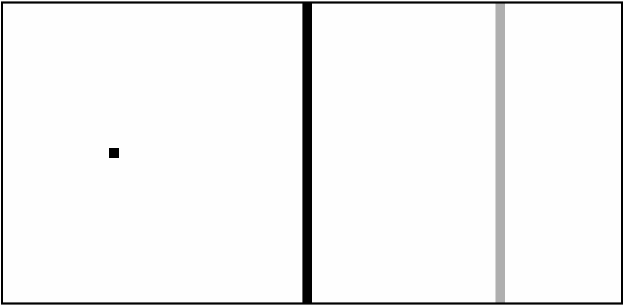
\includegraphics[scale=0.35]{Chapters/Images/synthetic_map.png}
     \caption{}
   \end{subfigure} 
   \begin{subfigure}[c]{.5\linewidth}
     \centering
     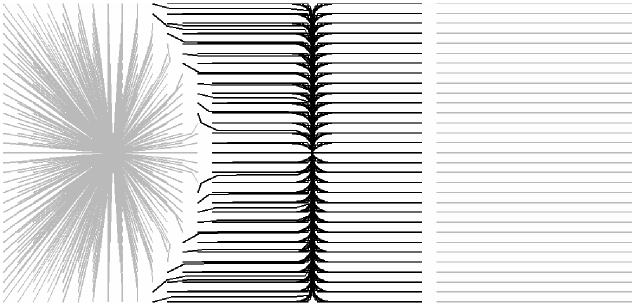
\includegraphics[scale=0.35]{Chapters/Images/synthetic_map_GVF.png}
     \caption{}
   \end{subfigure} \\
   
   \begin{subfigure}[c]{.5\linewidth}
     \centering
     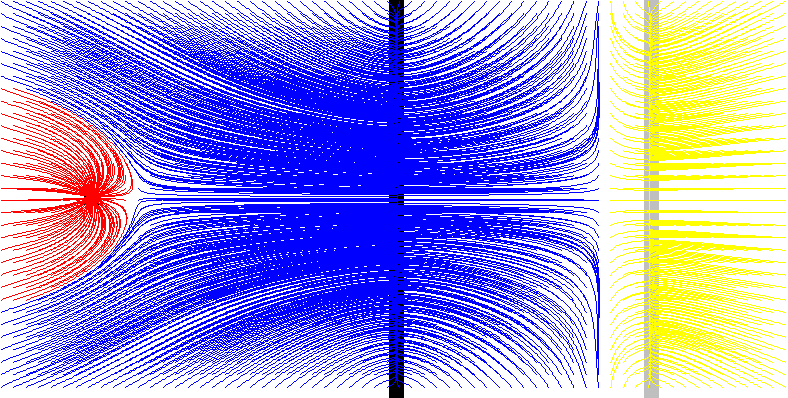
\includegraphics[scale=0.35]{Chapters/Images/synthetic_map_VFC_gamma017.png}
     \caption{}
   \end{subfigure}
   \begin{subfigure}[c]{.5\linewidth}
     \centering
     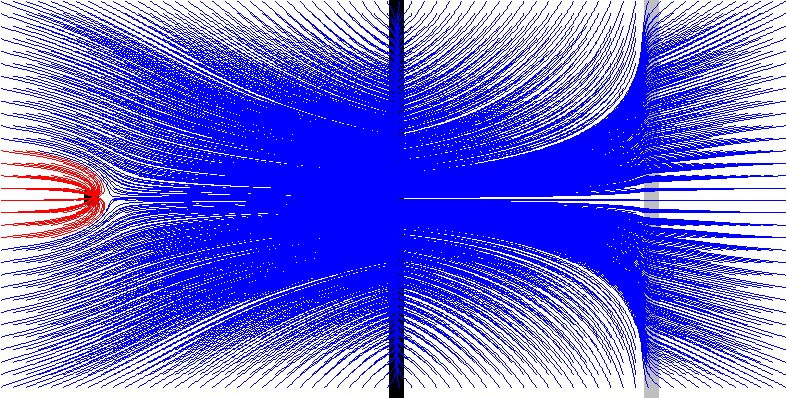
\includegraphics[scale=0.35]{Chapters/Images/synthetic_map_VFC_gamma011.png}
     \caption{}
   \end{subfigure}\\
   
   \caption{(a) Carte de contours $F(x,y)$ synthétique avec un bruit impulsionnel, un contour fort et un contour faible. Lignes d'attraction générées à partir (b) du champ GVF, (c) du champ VFC utilisant $m_1(x,y)$ avec $\gamma=1.7$ et (d) avec $\gamma = 1.1$ .}
   \label{fig:synthetic_map}
\end{figure}

\subsection{Mixed Vector Field Convolution}

 



\subsection{}
